\chapter{Development Methodology and Project Timeline}
\label{ch:methodology}

\section{Methodology}

The project follows an \textbf{iterative, incremental, checkpoint-driven}
development methodology. Work is organised as phases, each decomposed into
goals and tasks, and each meaningful unit of work ends in a validated,
documented, and committed checkpoint. The cycle used repeatedly throughout
development is:

\begin{center}
\small
\begin{tabular}{@{}c@{\qquad}c@{\qquad}c@{\qquad}c@{\qquad}c@{}}
Phase & $\rightarrow$ & Feature & $\rightarrow$ & Implementation \\
& $\rightarrow$ & Validation & $\rightarrow$ & Documentation \\
& $\rightarrow$ & Commit & $\rightarrow$ & Push \\
\end{tabular}
\end{center}

\noindent This style has two concrete consequences for the engineering process:

\begin{itemize}
  \item \textbf{Architecture decisions are recorded.} Seven architectural
  decisions (D1--D7) covering the permission model, role storage, the platform
  plane, academic structure, teacher/student assignments, resource scope, and
  session hardening were written down, decided, and then implemented in
  separate phases. A separate \textbf{documentation audit} (Phase~M) verified
  that the documents matched the code, rather than the reverse.
  \item \textbf{Validation is staged.} Schema changes are generated as
  Drizzle migrations, reviewed, and applied; TypeScript is type-checked; unit
  tests run on every change; database-backed integration suites run against
  PostgreSQL when available; and a human test-data (seeded demo) pass confirms
  user-observable behaviour before a phase is declared complete.
\end{itemize}

\noindent Scrum-like ceremonies are intentionally light: a single
product-oriented backlog (\texttt{docs/tasks.md}) holds the hierarchy, and the
project status file (\texttt{\seqsplit{docs/project-status.md}}) acts as the standing
checkpoint log so that work can resume across devices and sessions.

\section{Version Control and Continuity}

\noindent Work is committed to Git with conventional, scoped messages
(\texttt{feat(exams): publish to activate}) after each validated unit, and
pushed before interruptions (device switches, session ends). This makes the
repository itself the recovery protocol: any engineer can reconstruct the
state of the project from the tracker, status log, and Git history without
relying on conversation history.

\section{Project Timeline}

The project runs over Semester~V, from 1~July~2026 to 30~September~2026, in
seven planned phases. Table~\ref{tab:timeline} states the planned scope of each
phase and Figure~\ref{fig:gantt} renders the schedule as a Gantt chart.

\begin{table}[h]
\centering
\small
\begin{tabular}{@{}p{3.0cm}p{2.8cm}p{8.2cm}@{}}
\toprule
\textbf{Phase} & \textbf{Period (2026)} & \textbf{Planned scope} \\
\midrule
Analysis and planning & July 1--14 & Problem identification and requirement
analysis, study of academic guidelines, definition of scope and objectives. \\
System design & July 15--31 & System analysis, module decomposition,
architecture design (modular monolith), database schema design, technology
selection, project setup. \\
Core development & August 1--14 & Identity, tenancy, and authentication;
academic structure; material upload and the OCR processing pipeline. \\
Feature development & August 15--31 & AI-assisted syllabus structuring,
study-content generation, question bank, paper patterns, question papers, and
assessment authoring. \\
Examination and practice & September 1--14 & Scheduled assessments, student
attempts and evaluation, results and analytics, practice, export, and
interface hardening. \\
Testing and documentation & September 15--24 & Integration testing and
debugging, end-to-end validation, and project documentation. \\
Final review and submission & September 25--30 & Final review, correction, and
submission. \\
\bottomrule
\end{tabular}
\caption{Project timeline (Semester V, 2026).}
\label{tab:timeline}
\end{table}

\begin{figure}[h]
\centering
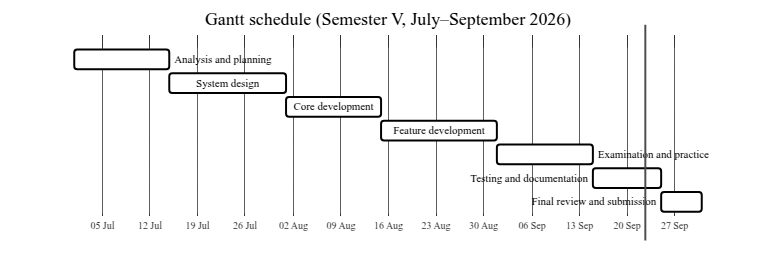
\includegraphics[width=\textwidth]{figures/gantt-chart.png}
\caption{Gantt chart of the seven project phases (July--September 2026).}
\label{fig:gantt}
\end{figure}

\section{Technologies Selected}

\noindent The technology stack, justified in detail in
Chapter~\ref{ch:implementation}, is summarised below: a TypeScript modular
monolith (NestJS) for the API; Next.js for the web client; PostgreSQL~17 with
Drizzle ORM as the single database; Redis for cache and RabbitMQ~3 for
messaging; a FastAPI OCR service and Python workers for heavy processing; a
provider-gateway integration for AI; Zod and Pydantic for schema validation at
the contract boundary; and Docker Compose plus a reverse proxy with a Cloudflare
Tunnel for deployment.